\documentclass{report}
\usepackage[utf8]{inputenc}
\usepackage{xcolor}
\usepackage{sectsty} %%Pour changer la couleur de la police 
\usepackage{listings}
\usepackage{amsmath}%%Pour les formules mathématique
\usepackage[final]{pdfpages}%%Pour l'inclusion de PDF

\title{Rapport}
\author{}
\date{}


\renewcommand{\contentsname}{Table des matières}
\renewcommand{\chaptername}{Chapitre}
\renewcommand{\listfigurename}{Liste des figures}
\renewcommand{\appendixname}{Annexe}
\renewcommand{\bibname}{Bibliographie}


\definecolor{bleurapport}{HTML}{00AAD4}

\chapterfont{\color{bleurapport}}
\sectionfont{\color{bleurapport}}
\subsectionfont{\color{bleurapport}}

\begin{document}


\includepdf{./PageGardeRapportTERM1.pdf}


\newpage
\null %%Pour faire une page vide
\newpage


\section*{Remerciements}
\hspace{0.5cm}Nous tenons tout d'abord à remercier Jimmy Lopez et Sébastien Beugnon pour nous avoir conseillés tout au long de notre projet.
	
	
	Nous remercions aussi nos tuteurs Guillaume Tisserant et Pierre Pompidor pour nous avoir accompagnés tout au long de la réalisation du projet, en particulier pour les choix des méthodes de profilage.

\newpage

\tableofcontents %%Table des matières

\newpage

\listoffigures %%Liste des figures

\newpage
\chapter*{Glossaire}

	\textit{Les termes définis dans ce glossaire sont identifiables dans le corps du texte au moyen d'un astérisque (*).}
	\bigbreak
	\begin{itemize}
	
	
		
		\item[\textbf{Bluff : }]Le bluff est une technique de jeu qui constiste à jouer comme si l'on possédait un jeu différent de celui détenu en réalité.\medskip
		
		\item[\textbf{Rationalité : }]La rationalité  appliquée au poker stipule que toutes les actions d'un joueur ont une logique.\medskip

		\item[\textbf{Agressité : }]	Un joueur agressif va jouer de façon à prendre l'initiative et continuer à miser dans le but d'intimider son adversaire et ainsi prendre l'avantage.	\medskip
		
		\item[\textbf{Profilage statique : }]Méthode consistant à profiler un joueur lors de chaque partie. Le profil établi n'est pas modifié à chaque fois que le joueur profilé effectue une action.\medskip
		
		\item[\textbf{Profilage dynamique : }]Méthode consistant à profiler un joueur tout au long d'une partie, en mettant à jour le profil établi en fonction des actions effectuées.\medskip
		
		\item[\textbf{Cave : }]La cave correspond à la somme possédée par chaque joueur au début de la partie.\medskip
		
		\item[\textbf{Pré-flop : }]Instant du jeu où le joueur possède deux cartes en main avant que les cartes communes n'aient été révélées.\medskip
		
		\item[\textbf{Flop : }]Correspond aux trois premières cartes communes posées sur la table.\medskip
		
		\item[\textbf{Checker : }]Correspond au moment où un joueur reste dans le jeu mais ne place pas d'enchères. Un joueur ne peut checker que si aucun joueur n'a misé avant lui.\medskip
		
		\item[\textbf{Dealer : }]Joueur se trouvant sur le siège d'où les cartes vont être distribuées.\medskip
		
		\item[\textbf{Blinde : }]Terme correspondant aux mises obligatoires pour les deux joueurs situés à gauche du dealer.\medskip
		
		\item[\textbf{Bouton : }]Le bouton représente le dealer qui distribue les cartes.\medskip
		
		\item[\textbf{Relancer : }]Une relance correspond au moment où un joueur va miser plus que ce que ses adversaires viennent de miser.\medskip
		
		\item[\textbf{Coup : }]Correspond à la distribution courante d'un jeu.\medskip
		
		\item[\textbf{Mise : }]Montant placé sur la table par un joueur à un instant donné.\medskip
		
		\item[\textbf{Se coucher : }]Correspond au moment où le joueur abandonne le coup. Ses mises sont alors perdues.\medskip
		
		\item[\textbf{Turn : }]Quatrième carte commune.\medskip
		
		\item[\textbf{River : }]Cinquième carte commune.\medskip
		
		\item[\textbf{Parler :}]Effectuer une action.\medskip
		
\end{itemize}



\chapter{Introduction}

\section{Généralités}
\hspace{0.5cm}Alors qu'actuellement, de plus en plus de méthodes de profilage sont établies dans le monde des jeux afin de trouver le profil d'un joueur adverse, le poker est un jeu qui pose problème dans ce domaine. En effet, ce jeu est basé sur la chance et sur le bluff. De ce fait, un joueur ne peut jamais être sûr à 100\% de pouvoir gagner et donc, son adversaire ne peut pas deviner le jeu qu'il a de manière certaine. C'est pourquoi, il est dur de profiler un joueur de manière certaine. Il y a donc des recherches dans le développement de méthodes permettant de profiler un joueur de manière efficace. \par

\section{Sujet}
\hspace{0.5cm}Le but de notre projet est de mettre en place une façon de profiler de façon efficace un joueur. Nous devrons tout d'abord établir une méthode de profilage statique. C'est à dire, une technique pour profiler un joueur en fonction des actions qu'il a effectuées pendant toute une partie, de manière globale. Après avoir implémenté cette première méthode de profilage, nous devrons mettre en place une intelligence artificielle pouvant jouer en fonction des résultats obtenus. Ainsi, nous pourrons voir si notre intelligence artificielle est capable de gagner plus de parties une fois le profil du joueur adverse établi.\par
S'il nous reste du temps, nous devrons mettre en place une méthode de profilage dynamique, avec par conséquent, un profil qui s’établit tout au long de la partie et qui est modifié à chaque nouvelle action du joueur adverse. Nous devrons alors, de même que précédemment, mettre en place une intelligence artificielle capable de jouer en exploitant les données de profilage. Ainsi, nous pourrons observer la différence du nombre de parties gagnées en fonction des deux types de profilage, à savoir, statique ou dynamique, mais aussi en fonction des profils établit. En effet, un joueur considéré comme agressif et rationnel est-il plus facile à profil et à battre qu'un joueur considéré comme non agressif et irrationnel ?\par

\section{Rapide description des règles du Texas Hold'Em Poker}
\subsection{Mise en place du jeu}
\hspace{0.5cm}Le Texas Hold'Em Poker est un jeu de cartes dans lequel le but d'un joueur est de gagner le plus d'argent. \par
Afin de commencer une partie, on désigne tout d'abord le bouton* qui sert à désigner le donneur ou dealer*. Le joueur choisi sera donneur pour une main, puis cela sera au tour du joueur à sa gauche une fois cette main terminée et ainsi de suite.  \par

Une fois le donneur sélectionné, il faut poser les blindes*. Le joueur directement à gauche du dealer* pose la petite blinde* alors que celui situé à sa gauche pose la grosse blinde* qui correspond souvent à exactement le double de la petite.\par

Le dealer* doit alors distribuer les cartes aux joueurs, à savoir, deux cartes par joueur. \par
\subsection{Préflop}
\hspace{0.5cm}Lorsque les cartes ont été distribuées, l'étape préflop* commence. Le tour de mises préflop* démarre donc par le joueur à la gauche de celui ayant mis la grosse blinde*. Celui-ci peut se coucher*, suivre* la grosse blinde* afin de pouvoir rentrer dans le coup ou encore relancer* d'un montant au moins égal à deux fois la grosse blinde*. Une fois le tour de mises préflop* terminé, on passe à l'étape suivante : le flop.\par

\subsection{Flop}
\hspace{0.5cm}Lors du flop*, le dealer* pose trois cartes faces apparentes au milieu de la table. Le premier tour de mises post-flop commence alors. Les règles sont les mêmes que lors du préflop* mis à part le fait que le premier joueur à parler* peut soit checker* soit miser*.\par

Une fois le tour de mises fini, on passe à l'étape du turn*.\par
\subsection{Turn}
Lors du turn*, le dealer* pose une carte découverte, à la suite des cartes du flop*. \par

Le troisième tour de mises commence alors. Celui-ci est identique au flop*.\par

Une fois celui-ci fini, on passe à la dernière étape, à savoir la river*.\par
\subsection{River}
\hspace{0.5cm}La dernière carte est alors posée par le dealer* au milieu, à la suite des autres cartes découvertes pendant les autres étapes. \par
De même que pour l'étape précédente, un tour de mises est effectué, avec les mêmes règles.\par
Une fois ce tour de mises terminé, les joueurs restants abattent leurs cartes et la meilleure main l'emporte.\par

\subsection{Les combinaisons}
\hspace{0.5cm}Lorsque l'on compare les mains au poker, la main gagnante est celle ayant la combinaison la plus forte. Au poker, il y a 9 combinaisons, de la quinte flush royale, correspondant à la combinaison la plus forte à la carte haute, correspondant à la combinaison la plus faible. Ainsi, une quinte flush royale gagne face à une quinte flush qui elle-même gagne contre un carré et caetera jusqu'à la combinaison la plus faible. \par


La combinaison la plus forte, la quinte flush royale est une suite d'une seule couleur, allant de l'as au dix. Par exemple, la main suivante correspond à une quinte flush royale. \par

		\begin{figure}[h]
			\begin{center}
				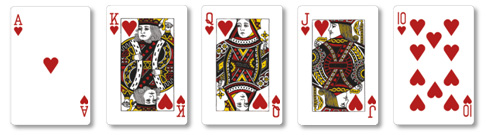
\includegraphics[scale=0.3]{./imagesRapport/quinteFlushRoyale.jpg}
			\end{center}
			\caption[Quinte Flush Royale]{Quinte Flush Royale}
		\end{figure}
		\medskip


Après la combinaison la plus forte, il y a la quinte flush, correspondant, comme on peut le voir dans la figure suivante, à une suite de cartes de la même couleur.\par

		\begin{figure}[h]
			\begin{center}
				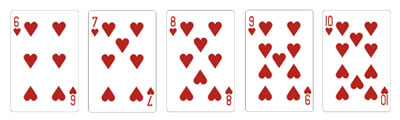
\includegraphics[scale=0.4]{./imagesRapport/quinteFlush.jpg}
			\end{center}
			\caption[Quinte Flush]{Quinte Flush}
		\end{figure}
		\medskip
\newpage
Par la suite, un joueur peut avoir un carré, à savoir, quatre cartes identiques. Si jamais deux joueurs ont un même carré, par exemple si le carré se trouve sur la table, le joueur gagnant sera celui ayant pour cinquième carte la carte la plus haute.\par 

		\begin{figure}[h]
			\begin{center}
				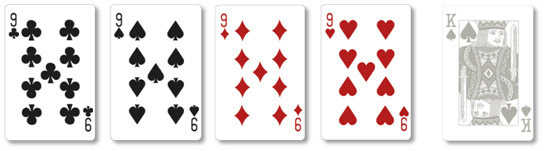
\includegraphics[scale=0.3]{./imagesRapport/carre.jpg}
			\end{center}
			\caption[Carré]{Carré}
		\end{figure}
		\medskip



Après le carré, vient le full qui correspond à trois cartes identiques et deux autres cartes identiques, comme on peut le voir dans la figure 1.4 suivante. \par


		\begin{figure}[h]
			\begin{center}
				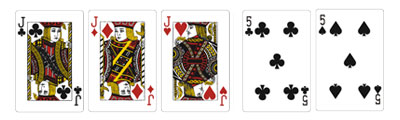
\includegraphics[scale=0.4]{./imagesRapport/full.jpg}
			\end{center}
			\caption[Full]{Full}
		\end{figure}
		\medskip

La combinaison correspondant à une couleur, ou flush, vient ensuite. Un joueur ayant une couleur doit donc avoir une main composée de cinq cartes de la même couleur.\par

		\begin{figure}[h]
			\begin{center}
				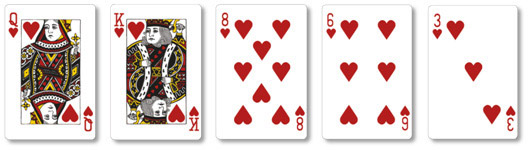
\includegraphics[scale=0.3]{./imagesRapport/couleur.jpg}
			\end{center}
			\caption[Couleur]{Couleur}
		\end{figure}
		\medskip

\newpage
Il y a ensuite une simple suite, donc une main composée de cartes qui se suivent, comme on peut le voir dans l'exemple suivant.\par

		\begin{figure}[h]
			\begin{center}
				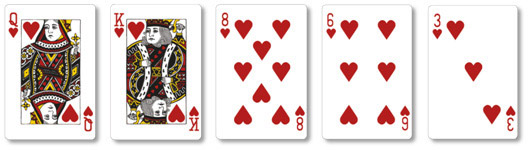
\includegraphics[scale=0.3]{./imagesRapport/suite.jpg}
			\end{center}
			\caption[Suite]{Suite}
		\end{figure}
		\medskip


Lorsqu'un joueur a un brelan, on compte uniquement ses trois cartes. Si jamais il y a égalité entre deux joueurs, on va regarder la carte haute suivante. Si celle-ci a de nouveau le même poids pour les deux joueurs, on regarde la deuxième carte la plus haute. La figure suivante correspond à un exemple de main ayant pour combinaison un brelan.\par
		\begin{figure}[h]
			\begin{center}
				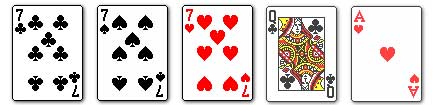
\includegraphics[scale=0.4]{./imagesRapport/brelan.jpg}
			\end{center}
			\caption[Brelan]{Brelan}
		\end{figure}
		\medskip
De même que précédemment, lorsqu'un joueur a une double paire, on compare les paires puis la carte haute. 
		\begin{figure}[h]
			\begin{center}
				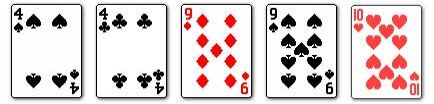
\includegraphics[scale=0.3]{./imagesRapport/doublePaire.jpg}
			\end{center}
			\caption[Double Paire]{Double Paire}
		\end{figure}
		\medskip

De même que pour la combinaison précédente, lorsqu'un joueur a une paire, si jamais il y a égalité entre deux joueurs pour la paire, on va comparer les cartes suivantes, en comparant chaque carte suivante. \par
\newpage
		\begin{figure}[h]
			\begin{center}
				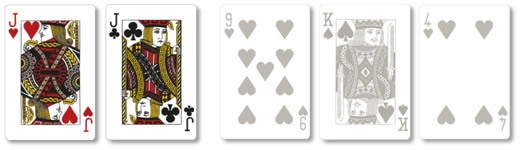
\includegraphics[scale=0.3]{./imagesRapport/paire.jpg}
			\end{center}
			\caption[Paire]{Paire}
		\end{figure}
		\medskip


Enfin, lorsqu'un joueur n'a pas d'autre combinaison, on va regarder sa carte la plus haute. De ce fait, si deux joueurs ont la même combinaison, une carte haute, et qu'ils ont la même carte haute, on va comparer la carte haute suivante et de même jusqu'à ce qu'on ait deux cartes différentes ou alors que l'on ait comparé les cinq cartes de la main. \par
		\begin{figure}[h]
			\begin{center}
				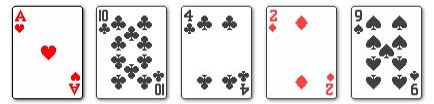
\includegraphics[scale=0.4]{./imagesRapport/carteHaute.jpg}
			\end{center}
			\caption[Carte Haute]{Carte Haute}
		\end{figure}
		\medskip

\section{Cahier des charges}
\subsection{Problématique}
\hspace{0.5cm}Durant les 10 semaines de développement du projet, nous devrons donc implémenter de façon intelligence une simple application permettant de jouer au poker puis, une intelligence artificielle capable de profiler différents types de joueur, tout d'abord de façon dynamique et éventuellement de façon statique. 
\subsection{Fonctionnalités obligatoires}

\hspace{0.5cm}Le projet qui nous a été attribué a pour but de développer une intelligence artificielle de poker permettant d'établir les différents profils des joueurs.\par
L'intelligence artificielle devra donc profiler ses adversaires en se basant sur différents critères comme la rationalité ou l'agressivité. Elle catégorisera alors les différents types de joueurs et leur attribuera des comportements.\par
Il nous est demandé d'établir dans un premier temps un profilage statique basé sur un automate à états finis, qui a pour but d'attribuer un unique comportement à chacun des joueurs pour toute la partie. Ce comportement sera attribué puis modifié après chaque nouvelle partie jouée contre un même joueur.\par
Par la suite, nous devrons mettre en place une nouvelle méthode de profilage afin de profiler de façon dynamique les joueurs. Dans cette seconde version, le profil d'un joueur sera mis à jour tout au long du déroulement d'une partie et l'intelligence artificielle devra pouvoir adapter son comportement aux réactions du joueur adverse.\par
Tout au long du développement, des scénarios de tests seront mis en place afin de vérifier le bon fonctionnement de la catégorisation des joueurs.\par

\subsection{Fonctionnalités optionnelles}

\hspace{0.5cm}Une fois les fonctionnalités obligatoires mises en place, il sera possible d'ajouter la possibilité d'avoir plus de deux joueurs dans une même partie, avec plusieurs intelligences artificielles ou plusieurs joueurs humains mais comprenant toujours au moins une intelligence artificielle.\par
On pourra également intégrer un système de dialogue entre les différents joueurs basé sur des phrases prédéfinies. Ainsi, chaque joueur, humain ou non, pourra envoyer des messages aux autres participants, et notre intelligence artificielle pourra utiliser ces messages pour mieux profiler ses opposants.\par 

\subsection{Spécifications techniques}

\hspace{0.5cm}Afin de faciliter les conditions de travail en groupe, il faudra utiliser un gestionnaire de version.\par
L'application devra être réalisée en utilisant le langage C++.\par
Le développement devra s'appuyer sur les méthodes agiles. Celles-ci sont basées sur une approche itérative dans un esprit collaboratif en prenant compte des besoins des utilisateurs et de leurs évolutions.\par

\subsection{Organisation prévisionnelle}

\hspace{0.5cm}Comme nous pouvons le voir dans l'annexe A représentant le diagramme de Gantt prévisionnel que nous avons mis en place. Dans un premier temps, nous avons donc prévu une étude préalable du sujet consistant à nous familiariser avec le vocabulaire du poker. De ce fait, Nous avons donc rapidement mis en place un glossaire contenant des définitions des différents termes. Pendant cette période, nous avons également défini les besoins des utilisateurs avec entre-autres un diagramme de cas d'utilisations. Durant cette période, nous avons aussi défini comment nous allions nous organiser durant le déroulement du projet, en définissant la fréquence des rendez-vous ainsi que les modalités de partage des données.\par
Par la suite, nous avons prévu de continuer par une étude détaillée durant laquelle nous allons élaborer un diagramme de classe, rédiger le cahier des charges ainsi que commencer à lire des articles sur le sujet.\par
Ensuite, nous passerons à une première étude technique durant laquelle nous commencerons par établir les normes de programmation. Puis, nous établirons une intelligence artificielle simple permettant à un joueur de jouer. Nous établirons par la suite les différents algorithmes et méthodes permettant d'établir un profilage statique du joueur adverse. Et nous établirons des jeux de tests. En même temps que cette étude technique, nous commencerons la phase de réalisation, en implémentant en parallèle l'interface graphique et l'intelligence artificielle simple puis, nous ajouterons la méthode de profilage statique et effectuerons les tests définis auparavant.\par
Nous effectuerons ensuite une seconde étude technique pendant laquelle nous définirons les méthodes et algorithmes qui seront utilisés afin d'implémenter la méthode de profilage dynamique. Dans ce même temps, nous implémenterons cette méthode de profilage dynamique, en effectuant les tests définis pendant la phase d'étude technique.\par
Enfin, la dernière partie sera réservée à la mise en place de la démonstration qui sera effectuée lors de la soutenance, ainsi qu'à la finalisation du rapport qui sera rédigé tout au long de la période du projet et à la préparation de la soutenance.\par

\chapter{Organisation du projet}



\section{Organisation du travail}

\section{Choix des outils de travail}
\subsection{Gestionnaire de versions}
\subsection{Création de l'interface graphique}
\subsection{Rédaction et mise en page du rapport}
\subsection{Normes de programmation}
\hspace{0.5cm}Nous coderons en français. Par conséquent, les différents identifiants des attributs, noms de classes et fonctions/méthodes que nous implémenterons auront des noms français, les méthodes toString ainsi que pour les accesseurs et mutateurs que nous nommerons getNomAttribut et setNomAttribut,
selon les conventions de codage établies.\par

Les noms des classes commenceront toujours par une majuscule suivie de minuscules. Si le nom de la classe est comp osé de plusieurs mots, alors on ajoutera une majuscule à chaque début de mot.\par

Les noms des méthodes, des variables et des attributs devront impérativement commencer par une minuscule avec une majuscule à chaque nouveau mot.\par

Pour l'indentation, il faudra mettre un maximum d'accolades, facilitant la reprise et l'ajout de code, même lorsque celles-ci ne sont pas obligatoires.\par

Des commentaires seront ajoutés pour chaque fonction et méthode, au dessus de la déclaration correspondante, dans les fichiers d'en-tête. Les commentaires des accesseurs et mutateurs ne sont pas obligatoires car explicites.
Dans ces commentaires seront précisés l'action de la fonction/méthode, l'ensemble des paramètres, l'élément retourné s'il existe. Ces commentaires seront de la forme suivante : \par

\begin{lstlisting}
/**
 *  @param
 *  @action
 *  @return
**/
\end{lstlisting}

Au début de chaque nouveau fichier créé, il faudra ajouter l'entête suivante: 
\begin{lstlisting}
/*========================================================================
Nom: fichier.cpp         Auteur: 
Maj:  27/03/2014         Creation: 01/02/2015
Projet: Profilage par essais et erreurs au poker
--------------------------------------------------------------------------
Specification: Specifications du fichier
=========================================================================*/
\end{lstlisting}

De plus, chaque commit effectué sur le projet Git devra avoir une description explicite permettant de savoir, sans avoir à parcourir le code, les modifications qui ont été apportées.\par

\subsection{Langage}
\hspace{0.5cm}Le langage utilisé pour la mise en place de l'application est le C/C++.

\chapter{Analyse du projet}

\section{Système de jeu}

\hspace{0.5cm}Afin de pouvoir effectuer le profilage d'un joueur, nous avons mis en place un jeu de poker à deux joueurs. Dans un premier temps, il s'agissait d'un joueur humain contre une intelligence artificielle ayant pour but de le profiler. Pour pouvoir jouer, une interface graphique a été mise en place pour permettre à la fois le suivi de la partie et le choix des actions.\par
Au départ, l'intelligence artificielle reposait sur un algorithme basique lui permettant de jouer une partie. Puis nous avons rapidement mis en place un calibrage de l'IA, afin de pouvoir lui attribuer un style de jeu (agressif, bluffeur...). Lors l'ajout de ce calibrage, nous avons complexifié le jeu de l'IA en prenant en compte le calibrage donné mais aussi en y ajoutant un choix d'action plus varié.\par
Afin de différencier les joueurs que l'IA profile, nous avons mis en place un système de pseudos. Avant le démarrage du jeu, il est alors possible de renseigner un pseudo, nouveau ou déjà existant, qui permet à l'IA de collecter et rassembler les données de profilage d'un même joueur. De ce fait, s'il se déconnecte et souhaite rejouer un autre jour, l'IA disposera toujours du précédent profilage effectué.\\

Par la suite, afin de permettre l'automatisation du profilage, et le lancements d'une série de parties, il nous a été demandé de revoir le système de jeu afin que l'IA existante puisse jouer contre une deuxième IA ne profilant pas. Dans cette version, l'interface n'est plus prise en compte et les deux intelligences jouent simultanément jusqu'à fin de la partie. Dans ce cas, un calibrage est donné pour cette deuxième IA, et celui-ci reste fixe pour la suite de parties. C'est l'IA qui profile qui va tenter de retrouver les valeurs de ce calibrage.\par
Pour permettre ces séries de tests, nous avons donc ajouté la possibilité de choisir le nombre de parties à lancer, afin de tester de façon efficace le profilage mis en place.

\section{Profilage}
%%On mettra ici les données communes aux profilages statiques et dynamiques
\subsection{Choix d'enregistrement des données}

\hspace{0.5cm}Afin de profiler nos joueurs, nous avons choisi d'enregistrer un certain nombre de données dans des fichiers de sortie. Selon le système de pseudos développé, nous avons décidé de mettre en place un fichier par joueur, représenté par le pseudo du joueur. Dans le but d'une réustilisation des données enregistrées par l'application, nous avons choisi le format de données Json car il a l'avantage d'être facilement exploitable. De plus, nous avons pu utiliser la librairie QJson pour traiter les données des fichiers.\\

Nous avons ensuite déterminé les données à prendre en compte au cours d'une partie, qui vont permettre le profilage du joueur adverse, et qui seront donc enregistrées dans les fichiers json.\par
Dans ce fichier, chaque valeur est représentée sous forme de taux, en pourcentage.\par
Au cours d'une partie, l'IA va donc enregister les chances de gain du joueur, au départ déduites de ses propres chances de gain, puis calculées si les cartes du joueur adverse sont dévoilées en fin de partie.\par
Elle va également calculer les différentes actions effectuées. Ici, nous avons choisi de classer les différentes actions en trois catégories, les suivis, les checks, et les mises qui comprennent aussi les relances. Chacune de ces valeurs représente donc le pourcentage de réalisation de cette action par le joueur en fonction du nombre de tours de jeu (par exemple si le joueur a suivi une fois sur deux, on aura 50\% de suivis). Si le joueur ne se couche pas, le total de ces trois valeurs est donc 100\%. Enfin un booléen indique si le joueur s'est couché ou non au cours de la partie.\par
Concernant les mises, afin d'être plus précis sur l'agressivité du joueur, nous mémorisons également la mise la plus haute effectuée en une fois par le joueur, ainsi que le total du montant misé sur l'ensemble des tours.\par
Finalement, le fichier contient tous les types de comportements possibles que l'on peut attribuer au joueur profilé. Nous avons choisi de catégoriser le joueur selon quatre critères : l'agressivité, c'est à dire sa capacité à miser, la rationalité, le bluff et la passivité. Ces quatre valeurs sont exprimées en pourcentage. Pour chacune d'elle nous avons déterminé une formule qui, à partir des données enregistrées dans le fichier et présentées plus haut, va calculer les taux associés. Pour l'agressivité, nous prenons en compte les mises effecutées, c'est à dire le nombre de mises, la mise la plus haute et le total des mises. La rationalité se base sur la cohérence entre les chances de gain du joueur et les mises effectuées. Puis nous avons dans un premier temps, calculé la passivité comme étant la somme du taux de checks et de suivis, soit l'inverse de l'agressivité, et le bluff comme l'inverse de la rationalité. Ces quatres valeurs prises deux à deux font donc 100\%.\par
Enfin, dans le but d'effectuer un profilage plus précis des joueurs, nous avons distingué chaque étape de jeu, et donc enregistré l'ensemble de ces valeurs pour les quatre étapes d'une partie : préflop, flop, turn et river. Un profil global de la partie est ensuite écrit avec les quatre valeurs de comportement. Puis un booléen contient le résultat de la partie.\\

Pour un joueur donné, le fichier contient donc l'ensemble des parties effectuées. Nous avons aussi au départ pensé à valoriser chacun des comportements de façon globale, après chaque partie enregistrée.


\subsection{Formule de calcul du taux de rationalité d'un joueur}

\hspace{0.5cm}Afin de calculer à combien de pourcentages un joueur a été rationnel pendant une partie, nous avons choisi de nous baser sur une courbe [ajouter un schéma de la courbe et l'expliquer] correspondant aux pourcentages théoriques de rationalité en fonction des chances de gagner. A partir de cette courbe, nous avons décidé de calculer la mise théorique que le joueur aurait dû miser en nous basant sur quatre paliers, comme on peut le voir dans la formule suivante. \par
Pour chaque palier, on regarde si les chances de gain du joueur sont comprises entre g1 et g2. Une fois le palier trouvé, on calcule la mise théorique, en sachant que celle-ci sera comprise entre les m1 et m2 correspondant au palier. \par
	Gain = chances de gain du joueur,\\
	Ra = rationalité\\
	$M_{th}$ = Mise théorique.\\

\small{
\begin{align*}
	M_{th} = \left((Gain - g1) * \left(\frac{m2-m1}{g2-g1}\right)\right)+m1
	\begin{cases}
		Ra \in [m1=0 - m2=10] &\text{Si Gain} \in [g1=0 - g2=30]\\
		Ra \in [m1=11 - m2=25] &\text{Si Gain} \in [g1=31 - g2=50]\\
		Ra \in [m1=26 - m2=65] &\text{Si Gain} \in [g1=51 - g2=69]\\
		Ra \in [m1=66 - m2=100] &\text{Si Gain} \in [g1=70 - g2=100]\\
	\end{cases}
\end{align*}
}

Après avoir calculé la mise théorique que le joueur aurait dû faire, nous la comparons avec la mise réelle du joueur. On obtient alors la formule suivante pour calculer la rationalité : \par

\begin{align*}
Rationalit\acute{e} = 100-abs(M_{th}-M_{r\acute{e}elle})
\end{align*}

\subsection{Formule de calcul du taux d'agressivité d'un joueur}

\hspace{0.5cm}Afin de calculer le pourcentage d'agressivité d'un joueur pendant une partie, de même que pour la rationalité, nous avons choisi de nous baser sur un système de paliers, en prenant en compte trois paramètres : le pourcentage de mises, le total des mises qui est exprimé en pourcentage de jetons par rapport aux jetons de départ du joueur et, la mise la plus haute du joueur, elle aussi exprimée en pourcentage de jetons par rapport aux jetons de base.\par
De même que précédemment, pour chaque palier, on va regarder si la mise la plus haute (mph) est comprise entre mph1 (mise la plus haute 1) et mph2. Une fois le palier trouvé, on calcule le pourcentage d'agressivité théorique qui sera compris entre ag1 et ag2. \par


\small{
\begin{align*}
	Ag_{th}=
	\begin{cases}
		Ag_{th} \in [0-50] Si mph \in [0-25] &\text{ratio1}=\frac{1}{2} \text{ ratio2}=\frac{1}{2} \\
		Ag_{th} \in [51-80] Si mph \in [26-50] &\text{ratio1}=\frac{2}{3} \text{ ratio2}=\frac{1}{3} \\
		Ag_{th} \in [81-100] Si mph \in [51-100]  &\text{ratio1}=\frac{2}{3} \text{ ratio2}=\frac{1}{3}\\
	\end{cases}
\end{align*}

}

Pour calculer le pourcentage théorique d'agressivité, on se base sur la formule suivante, en sachant que pour chaque palier, nous accordons des poids différents au total des mises et au nombre de mises.\par

\begin{align*}
	&0<y<mph2-ag2\\
	&x=ratio1 * nbMises + ratio2 * totalMises\\
	&y=\left(x*\frac{mph2-ag2}{100}\right)
\end{align*}

Pour le dernier palier, nous ne nous basons pas sur la formule précédente mais sur la formule suivante :\\ 

\begin{align*}
	y=\left(x*\frac{100-mph}{100}\right)
\end{align*}

\subsection{Formule de calcul du taux de bluff d'un joueur}

\hspace{0.5cm}Étant donné le fait que nous partons du principe que le bluff est l'inverse de la rationalité, nous calculons le taux de bluff en utilisant la formule suivante : \par

\begin{align*}
	bluff=100-rationalit\acute{e}
\end{align*}


\subsection{Formule de calcul du taux de passivité d'un joueur}

\hspace{0.5cm}Nous avons décidé que le taux de passivité d'un joueur se calcule en fonction du nombre de fois où il a suivi et du nombre de fois où il a checké. De ce fait, nous avons choisi d'établir la formule suivante pour calculer le taux de passivité d'un joueur : \par
\begin{align*}
	passivit\acute{e}=tauxChecks+tauxSuivis
\end{align*}


\section{Profilage statique}

\section{Réutilisation des résultats du profilage}

\section{Profilage dynamique}

\section{Réutilisation des résultats du profilage}


\chapter{Mise en place des méthodes de profilage}

\section{Calibrage des intelligences artificielles}

\hspace{0.5cm}Afin de pouvoir choisir les taux d'agressivité et de rationalité de l'IA profilée, et pour pouvoir faire varier le comportement de celle qui le profile, il nous a fallu mettre en place un calibrage des intelligences artificielles. C'est à dire qu'à partir de taux d'agressivité et de rationalité données, une IA doit pouvoir, quand c'est à elle de jouer, choisir une action en adéquation avec les valeurs fournies. Une intelligence aritificielle agressive aura donc tendance à fortement miser.\\

Pour notre première version de l'intelligence artificielle avec un calibrage, nous avons choisi de calculer une action pour chaque paramètre du calibrage, donc une action d'agressivité et une action de rationalité. Puis nous avons mis en place une méthode de sélection à partir des deux actions calculées et des taux de calibrage correspondants.\par
Pour le choix de l'action agressive, le calcul se base sur une mise théorique d'agressivité en fonction des même paliers établis que pour le profilage. Puis afin de respecter le pourcentage d'agressivité donné pour l'IA, nous avons dans un premier temps pensé à alterner entre action agressive et action passive en fonction du calibrage. En effet, le profilage de l'agressivité s'effectue selon trois critères, la fréquence de mises, la mise la plus haute et le montant total des mises. De ce fait, afin que notre IA ne mise pas de façon constante, nous avons pensé à générer un nombre aléatoire entre un et cent et le comparer au taux d'agressivité donné pour choisir l'action. Par exemple, si le calibrage d'agressivité vaut 70\%, alors si le nombre aléatoire est compris entre 0 et 70, on effectue une action de mise cohérente selon la mise théorique (une mise, une relance ou un suivi selon la situation), et si au contraire le nombre est compris entre 70 et 100, on choisit une action passive.\par
Le choix de l'action rationelle est basé sur le même principe. La mise théorique de rationalité est calculée en fonction des chances de gain de l'IA, puis de la même manière que pour l'agressivité, un nombre aléatoire détermine si on effectue une action rationelle ou non. Si on a une valeur de rationalité entre 0 et le taux alors on choisit une action rationelle, qui correspond à la mise théorique et qui varie selon la situation actuelle du jeu. Sinon, on liste l'ensemble des actions irrationelles, comme une mise en dessous ou en dessus de la mise théorique, puis pour renforcer l'irationnalité, et donc l'imprévisibilité du joueur, la sélection de l'action parmi toutes celles considérées comme irrationelles se fait de façon aléatoire.\par
Enfin, une fois les deux actions calculées, une sélection aléatoire était faite entre ces deux actions, avec les chances de sélection proportionnelles aux valeurs de calibrage.\\

\hspace{0.5cm}Par la suite nous avons revu le calibrage de l'agressivité qui n'était pas assez précis. En effet, tout comme pour calibrer la rationalité, nous laissions une part de hasard dans le calcul de l'action de l'intelligence artificielle. Ceci avait pour effet de produire des résultats trop imprévisibles, et parfois trop éloignés du calibrage de départ.\par
Pour pallier ce problème, nous avons calculé une action de mise correspondante au taux d'agressivité en fonction de la mise totale effectuée par l'intelligence artificielle au cours de la partie. Nous avons également adapté le calcul côté profilage afin que la mise totale devienne le critère principal, et plus la mise la plus haute.\par
A chaque tour, le résolveur calcule donc la mise théorique à effectuer selon les nouveaux paliers.\par

	Ag.		Mise totale

	0 – 50		0 – 25	exclu
	50 – 80		25 – 60 exclu
	80 – 100	60 – 100 exclu
	100			100

Selon le calibrage, le but est donc que l'intelligence artificielle effectue la mise prévue. Seulement, il n'est pas possible de déterminer la durée de la partie. Il faut donc que celle-ci effectue progressivement sa mise, sans terminer trop tôt où elle devra effectuer des actions check ou suivi pour terminer, ce qui diminuera le taux d'agressivité; et ni trop tard pour qu'elle puisse être considérée suffisamment agressive.\par
Pour ce faire, nous misons de façon croissante, depuis un départ minimum, jusqu'à atteindre la mise théorique totale calculée à partir du calibrage.\par
En prenant un rapport $\times2$, on obtient donc les mises totales suivantes à chaque tour de jeu.\par
Ex : 	5 – 10 – 20 – 40 – 80 		avec 80 mise totale théorique.

Dans ce cas, cela revient donc à miser 5; 5; 10; 20 puis 40.

Afin d'obtenir ce résultat, nous différencions deux cas : celui où l'intelligence artificielle peut miser et celui où elle doit suivre/relancer ou se coucher.\par
Si elle peut miser, alors elle joue la mise théorique courante en faisant attention de ne pas dépasser la mise théorique totale. Dans le cas où on est au river (dernier tour), alors elle mise directement ce qu'il lui manque pour arriver à cette mise théorique totale.\par

Dans le cas où l'adversaire a misé/relancé, alors l'intelligence artificielle va comparer la mise théorique courante avec la mise adverse et la valeur de relance minimum. Dans le cas où le mise théorique est inférieure à la valeur de suivi -10\% alors on se couche, pour ne  pas miser trop haut en suivant. Si celle-ci est comprise entre le taux de suivi $\pm$ 10\%, on suit.
Dans le cas ou la relance est $\leq$ à la valeur à miser +10\% , on relance de la valeur la plus proche de la mise théorique. Sinon on suit.\par


A la suite de ces changements nous avons également revu la sélection entre les actions d'agressivité et de rationalité, une fois ces deux dernières calculées.\par

Une fois que le calibrage nous a donné l'action agressive et l'action rationnelle, on effectue une fusion entre les deux. Dans les cas où les deux actions sont identiques, l'action est prise. Si ce sont toutes les deux des mises/relances, on prend la moitié des du nombre de jetons, proportionnellement aux pourcentages de calibrage.
Enfin, il reste la possibilité que les actions soient différentes. Ici on distingue deux cas :
\begin{itemize}
\renewcommand{\labelitemi}{-}
\item on arrive à déterminer une action représentant un juste milieu, par exemple si les deux actions sont se coucher et relancer, on fait suivre l'intelligence artificielle. Dans le cas où on a checker / miser, on considère l'action checker comme miser 0 et on effectue le calcul de la mise moyenne expliqué ci-dessus.
\item sinon on tire aléatoirement l'action parmi les deux, toujours en prenant en compte les pourcentages du calibrage.

\end{itemize}

\section{Profilage statique}
\subsection{Scénarios de tests}

\hspace{0.5cm}Afin de pouvoir évaluer le profilage effectué par l'IA, il nous a été conseillé de se baser sur la différence entre l'action attendue du joueur adverse, puis son action réelle. De ce fait, il est possible de déterminer facilement l'efficacité du profilage, en analysant cette différence entre l'attendu et le réel.\par
Pour que l'IA puisse connaître le comportement attendu d'un joueur à partir d'une situation donnée, nous avons établi l'ensemble des scénarios possibles. Chaque scénario se base sur le calibrage de l'IA qui profile (son agressivité), ainsi que ses chances de gain. Pour chacune de ces situations, on établit le comportement attendu rationellement par le joueur adverse, exprimé sous forme de taux d'agressivité. Ce sont ces données que l'IA va utiliser pour calculer la différence des actions attendues et réelles.\\

\subsection{Test du profilage}

\hspace{0.5cm}Afin d'obtenir un résultat des données de profilage au bout de plusieurs parties, nous enregistrons à la fin de chaque partie une ligne de résultats dans un fichier csv à partir des données du json. Cette ligne contient la situation du jeu (calibrage IA et chances de gain), les taux d'agressivité et rationalité attendus, les taux réels et la distance entre ces deux. Enfin une moyenne des taux attendus est mise à jour à chaque ajout, c'est elle qui va donner le profilage obtenu au bout de x parties.\par
Cela va donc permettre le lancement de plusieurs parties, IA contre IA, pour obtenir un profilage rapidement. Suite à ces résultats, il est alors possible de réaliser des courbes permettant d'observer la convergeance entre le profil établi, et le calibrage de l'IA profilée. La distance doit alors être de plus en plus proche de zéro.


\subsection{Établissement des profils attendus}

\hspace{0.5cm}Pour calculer une action attendue, c'est à dire un taux d'agressivité et de rationalité attendu pour le joueur, l'IA utilise lors des premières parties les scénarios de tests étalis.\par
Mais une fois le profilage lancé, et les premiers résultats obtenus, la méthode de profilage peut alors commencer à se servir des situations précédentes pour calculer l'action attendue d'un joueur. En effet, selon la situation, il est possible de déterminer quelle va être l'action du joueur en se référant aux scénarios de tests conçus, qui sont communs à tous les joueurs, mais également en se référant aux parties précédentes, si l'on a déjà testé sa réaction précédemment dans une situation équivalente. Une situation équivalente est ici considérée à partir du taux d'agressivité du joueur adverse au joueur, donc l'IA qui profile, et des chances de gain du joueur. A partir de cette méthode, la valeur d'une action réelle dans une situation va permettre de donner la valeur d'une action attendue dans une prochaine partie. Cette méthode va ici nous permettre de profiler le joueur plus rapidement, en réutilisant les réultats précédents.\par
Pour effectuer cette réutilisation, plusieurs méthodes ont été considérées. Tout d'abord, celle qui cherche la situation la plus proche, selon l'agressivité du profileur et les chances de gain, sans considérer le taux de somilarité entre les deux situations. C'est à dire que dans cette version, les valeurs de l'action attendue correspondent aux valeurs des scénarios de tests uniquement pour la première partie, par la suite c'est la valeur précédente la plus proche qui est prise en compte.\par
Une seconde méthode a été de limiter la réutilisation des actions réelles comme action attendues en considérant l'équivalence entre les parties. Toujours en prenant en compte les valeurs d'agressivité et des chances de gain, les pourcentages doivent alors ne varier que de 10\% maximum par exemple, pour que l'on puisse considérer la situation comme équivalente, et donc considérer les actions effectuées comme action attendues pour la partie courante. Ici on prend toujours la situation la plus proche, mais seulement parmi les parties dites équivalentes. Et donc dans le cas où les valeurs sont trop éloignées, on se réfère aux scénarios de tests.\par
Enfin, il est aussi possible de prendre une situation dans laquelle la distance est la plus petite.

\subsection{Réutilisation des résultats du profilage}

\hspace{0.5cm}Une fois un profil établi, nous pouvons alors faire jouer l'IA en fonction dans le but de lui faire gagner le plus de parties possibles. Lors de cette étape le profilage est interrompu, et on utilise le comportement déduit pour calibrer l'IA de façon à ce qu'elle puisse gagner face à ce type de joueur.\par
Pour une première version, nous avons choisi de seulement prendre en compte le profil final établi et d'attribuer un calibrage selon divers paliers. Ici on prend en compte trois paliers pour l'agressivité ainsi que pour la rationalité. De 0 à 40\% pour le premier palier, 40 à 60\% pour une valeur moyenne puis de 60 à 100\% pour la palier haut. Nous avons déduit les calibrage correspondants à chaque palier du joueur profilé, les résultats sont présentés dans le tableau suivant.\\


\section{Profilage dynamique}
\subsection{Scénarios de tests}
\subsection{Établissement des profils attendus}
\subsection{Réutilisation des résultats du profilage}


\chapter{Analyse des résultats obtenus}

\section{Profilage statique}
\subsection{Scénarios de tests}
\subsection{Analyse des gains de parties}

\section{Profilage dynamique}
\subsection{Analyse des gains de parties}


\chapter{Perspectives et conclusion}
\section{Perspectives d'amélioration du profilage}
\section{Profilage obtenu}

%%bibliographie /sitographie

\bibliographystyle{plain}
\nocite{*}
\bibliography{biblio}

%%Annexes
\appendix
\chapter{Test annexe}

\end{document}
